% ID: 61225
\graphicspath{ {./bst-insertion-removal-images/} }

\question Suppose that we have the following binary search tree:

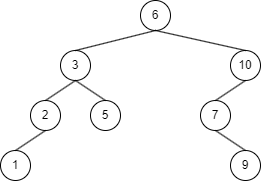
\includegraphics[scale=0.75]{topics/trees/binary-search-trees/medium/bst-insertion-removal-images/start.png}

Remember that BSTs do not allow copies. Draw the final tree after we perform the following operations:
\begin{lstlisting}
 
    insert(2);
    insert(11);
    insert(8);
    insert(4);
    remove(2);
    remove(6);
\end{lstlisting}

\begin{solution}
\lstinline{insert(2)}:

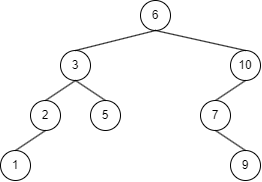
\includegraphics[scale=0.75]{topics/trees/binary-search-trees/medium/bst-insertion-removal-images/insert2.png}

\lstinline{insert(11)}:

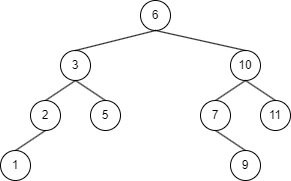
\includegraphics[scale=0.75]{topics/trees/binary-search-trees/medium/bst-insertion-removal-images/insert11.png}

\lstinline{insert(8)}:

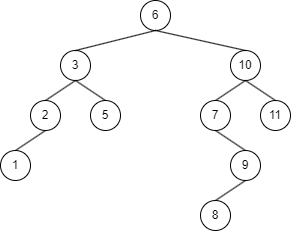
\includegraphics[scale=0.75]{topics/trees/binary-search-trees/medium/bst-insertion-removal-images/insert8.png}

\lstinline{insert(4)}:

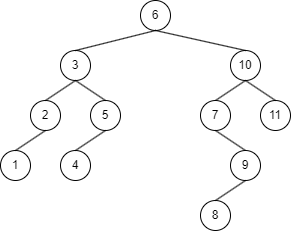
\includegraphics[scale=0.75]{topics/trees/binary-search-trees/medium/bst-insertion-removal-images/insert4.png}

\lstinline{remove(2)}:

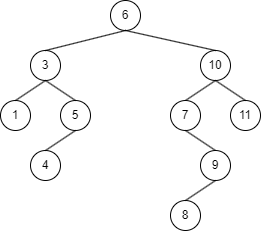
\includegraphics[scale=0.75]{topics/trees/binary-search-trees/medium/bst-insertion-removal-images/remove2.png}

\lstinline{remove(6)}--Hibbard deletion promotes a member of the left subtree:

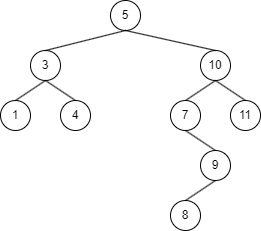
\includegraphics[scale=0.75]{topics/trees/binary-search-trees/medium/bst-insertion-removal-images/remove6.png}

Alternate solution after \lstinline{remove(6)}--Hibbard deletion promotes a member of the right subtree:

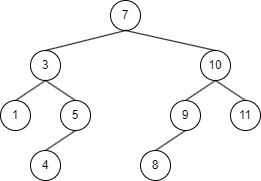
\includegraphics[scale=0.75]{topics/trees/binary-search-trees/medium/bst-insertion-removal-images/remove6_2.png}
\end{solution}
